% Options for packages loaded elsewhere
\PassOptionsToPackage{unicode}{hyperref}
\PassOptionsToPackage{hyphens}{url}
\PassOptionsToPackage{dvipsnames,svgnames,x11names}{xcolor}
%
\documentclass[
  number,
  preprint,
  3p]{elsarticle}

\usepackage{amsmath,amssymb}
\usepackage{iftex}
\ifPDFTeX
  \usepackage[T1]{fontenc}
  \usepackage[utf8]{inputenc}
  \usepackage{textcomp} % provide euro and other symbols
\else % if luatex or xetex
  \usepackage{unicode-math}
  \defaultfontfeatures{Scale=MatchLowercase}
  \defaultfontfeatures[\rmfamily]{Ligatures=TeX,Scale=1}
\fi
\usepackage{lmodern}
\ifPDFTeX\else  
    % xetex/luatex font selection
\fi
% Use upquote if available, for straight quotes in verbatim environments
\IfFileExists{upquote.sty}{\usepackage{upquote}}{}
\IfFileExists{microtype.sty}{% use microtype if available
  \usepackage[]{microtype}
  \UseMicrotypeSet[protrusion]{basicmath} % disable protrusion for tt fonts
}{}
\makeatletter
\@ifundefined{KOMAClassName}{% if non-KOMA class
  \IfFileExists{parskip.sty}{%
    \usepackage{parskip}
  }{% else
    \setlength{\parindent}{0pt}
    \setlength{\parskip}{6pt plus 2pt minus 1pt}}
}{% if KOMA class
  \KOMAoptions{parskip=half}}
\makeatother
\usepackage{xcolor}
\setlength{\emergencystretch}{3em} % prevent overfull lines
\setcounter{secnumdepth}{5}
% Make \paragraph and \subparagraph free-standing
\ifx\paragraph\undefined\else
  \let\oldparagraph\paragraph
  \renewcommand{\paragraph}[1]{\oldparagraph{#1}\mbox{}}
\fi
\ifx\subparagraph\undefined\else
  \let\oldsubparagraph\subparagraph
  \renewcommand{\subparagraph}[1]{\oldsubparagraph{#1}\mbox{}}
\fi


\providecommand{\tightlist}{%
  \setlength{\itemsep}{0pt}\setlength{\parskip}{0pt}}\usepackage{longtable,booktabs,array}
\usepackage{calc} % for calculating minipage widths
% Correct order of tables after \paragraph or \subparagraph
\usepackage{etoolbox}
\makeatletter
\patchcmd\longtable{\par}{\if@noskipsec\mbox{}\fi\par}{}{}
\makeatother
% Allow footnotes in longtable head/foot
\IfFileExists{footnotehyper.sty}{\usepackage{footnotehyper}}{\usepackage{footnote}}
\makesavenoteenv{longtable}
\usepackage{graphicx}
\makeatletter
\def\maxwidth{\ifdim\Gin@nat@width>\linewidth\linewidth\else\Gin@nat@width\fi}
\def\maxheight{\ifdim\Gin@nat@height>\textheight\textheight\else\Gin@nat@height\fi}
\makeatother
% Scale images if necessary, so that they will not overflow the page
% margins by default, and it is still possible to overwrite the defaults
% using explicit options in \includegraphics[width, height, ...]{}
\setkeys{Gin}{width=\maxwidth,height=\maxheight,keepaspectratio}
% Set default figure placement to htbp
\makeatletter
\def\fps@figure{htbp}
\makeatother

\usepackage{booktabs}
\usepackage{longtable}
\usepackage{array}
\usepackage{multirow}
\usepackage{wrapfig}
\usepackage{float}
\usepackage{colortbl}
\usepackage{pdflscape}
\usepackage{tabu}
\usepackage{threeparttable}
\usepackage{threeparttablex}
\usepackage[normalem]{ulem}
\usepackage{makecell}
\usepackage{xcolor}
\usepackage{algorithm}
\makeatletter
\@ifpackageloaded{tcolorbox}{}{\usepackage[skins,breakable]{tcolorbox}}
\@ifpackageloaded{fontawesome5}{}{\usepackage{fontawesome5}}
\definecolor{quarto-callout-color}{HTML}{909090}
\definecolor{quarto-callout-note-color}{HTML}{0758E5}
\definecolor{quarto-callout-important-color}{HTML}{CC1914}
\definecolor{quarto-callout-warning-color}{HTML}{EB9113}
\definecolor{quarto-callout-tip-color}{HTML}{00A047}
\definecolor{quarto-callout-caution-color}{HTML}{FC5300}
\definecolor{quarto-callout-color-frame}{HTML}{acacac}
\definecolor{quarto-callout-note-color-frame}{HTML}{4582ec}
\definecolor{quarto-callout-important-color-frame}{HTML}{d9534f}
\definecolor{quarto-callout-warning-color-frame}{HTML}{f0ad4e}
\definecolor{quarto-callout-tip-color-frame}{HTML}{02b875}
\definecolor{quarto-callout-caution-color-frame}{HTML}{fd7e14}
\makeatother
\makeatletter
\makeatother
\makeatletter
\makeatother
\makeatletter
\@ifpackageloaded{caption}{}{\usepackage{caption}}
\AtBeginDocument{%
\ifdefined\contentsname
  \renewcommand*\contentsname{Table of contents}
\else
  \newcommand\contentsname{Table of contents}
\fi
\ifdefined\listfigurename
  \renewcommand*\listfigurename{List of Figures}
\else
  \newcommand\listfigurename{List of Figures}
\fi
\ifdefined\listtablename
  \renewcommand*\listtablename{List of Tables}
\else
  \newcommand\listtablename{List of Tables}
\fi
\ifdefined\figurename
  \renewcommand*\figurename{Figure}
\else
  \newcommand\figurename{Figure}
\fi
\ifdefined\tablename
  \renewcommand*\tablename{Table}
\else
  \newcommand\tablename{Table}
\fi
}
\@ifpackageloaded{float}{}{\usepackage{float}}
\floatstyle{ruled}
\@ifundefined{c@chapter}{\newfloat{codelisting}{h}{lop}}{\newfloat{codelisting}{h}{lop}[chapter]}
\floatname{codelisting}{Listing}
\newcommand*\listoflistings{\listof{codelisting}{List of Listings}}
\makeatother
\makeatletter
\@ifpackageloaded{caption}{}{\usepackage{caption}}
\@ifpackageloaded{subcaption}{}{\usepackage{subcaption}}
\makeatother
\makeatletter
\@ifpackageloaded{tcolorbox}{}{\usepackage[skins,breakable]{tcolorbox}}
\makeatother
\makeatletter
\@ifundefined{shadecolor}{\definecolor{shadecolor}{rgb}{.97, .97, .97}}
\makeatother
\makeatletter
\makeatother
\makeatletter
\makeatother
\journal{Journal of Multivariate Analysis}
\ifLuaTeX
  \usepackage{selnolig}  % disable illegal ligatures
\fi
\usepackage[]{natbib}
\bibliographystyle{elsarticle-num-names}
\IfFileExists{bookmark.sty}{\usepackage{bookmark}}{\usepackage{hyperref}}
\IfFileExists{xurl.sty}{\usepackage{xurl}}{} % add URL line breaks if available
\urlstyle{same} % disable monospaced font for URLs
\hypersetup{
  pdftitle={Studying the Performance of the Jellyfish Search Optimiser for the Application of Projection Pursuit},
  pdfauthor={H. Sherry Zhang; Dianne Cook; Nicolas Langrené; Jessica Wai Yin Leung},
  pdfkeywords={projection pursuit, Jellyfish Search Optimiser
(JSO), Optimisation},
  colorlinks=true,
  linkcolor={blue},
  filecolor={Maroon},
  citecolor={Blue},
  urlcolor={Blue},
  pdfcreator={LaTeX via pandoc}}

\setlength{\parindent}{6pt}
\begin{document}

\begin{frontmatter}
\title{Studying the Performance of the Jellyfish Search Optimiser for
the Application of Projection Pursuit}
\author[1]{H. Sherry Zhang%
\corref{cor1}%
}
 \ead{huize.zhang@austin.utexas.edu} 
\author[2]{Dianne Cook%
%
}
 \ead{dicook@monash.edu} 
\author[3]{Nicolas Langrené%
%
}
 \ead{nicolaslangrene@uic.edu.cn} 
\author[2]{Jessica Wai Yin Leung%
%
}
 \ead{Jessica.Leung@monash.edu} 

\affiliation[1]{organization={University of Texas at Austin, Department
of Statistics and Data Sciences},city={Austin},country={United
States},countrysep={,},postcode={78751},postcodesep={}}
\affiliation[2]{organization={Monash University, Department of
Econometrics and Business
Statistics},city={Melbourne},country={Australia},countrysep={,},postcode={3800},postcodesep={}}
\affiliation[3]{organization={BNU-HKBU United International
College, Department of Mathematical
Sciences},city={Zhuhai},country={China},countrysep={,},postcode={519087},postcodesep={}}

\cortext[cor1]{Corresponding author}




        
\begin{abstract}
Projection pursuit (PP) is a dimension reduction technique that
identifies low-dimensional projections in high-dimensional data by
optimising a criteria function known as the PP index. The optimisation
in PP can be non-smooth and requires identifying optima with a small
``squint angle'', detectable only from close proximity. To address these
challenges, this study investigates the performance of a recent
swarm-based algorithm, Jellyfish Search Optimiser (JSO), for optimising
PP indexes. The performance of JSO is evaluated across various
hyper-parameter settings and compared with existing optimisers.
Additionally, this work proposes novel methods to quantify two
properties of the PP index -- smoothness and squintability -- that
capture the complexities inherent in PP optimisation problems. These two
metrics are evaluated with JSO hyper-parameters to determine their
effect on JSO success rate. The JSO algorithm has been implemented in
the \texttt{tourr} package, while calculations for smoothness and
squintability are available in the \texttt{ferrn} package.
\end{abstract}





\begin{keyword}
    projection pursuit \sep Jellyfish Search Optimiser (JSO) \sep 
    Optimisation
\end{keyword}
\end{frontmatter}
    \ifdefined\Shaded\renewenvironment{Shaded}{\begin{tcolorbox}[enhanced, interior hidden, frame hidden, boxrule=0pt, borderline west={3pt}{0pt}{shadecolor}, breakable, sharp corners]}{\end{tcolorbox}}\fi

\textbf{README}:

\begin{itemize}
\item
  British English (``American or British usage is accepted, but not a
  mixture of these'')*
\item
  No ``we'' - always third person
\item
  Check if the affiliation information is correct
\item
  word use:

  \begin{itemize}
  \tightlist
  \item
    Use jellyfish search optimiser, or JS optimiser, not jellyfish
    optimiser (my bad for leading the way)
  \item
    ``hyper-parameter'' rather than ``hyperparameter''
  \end{itemize}
\end{itemize}

\hypertarget{introduction-nicolas-and-jessica}{%
\section{Introduction {[}Nicolas and
Jessica{]}}\label{introduction-nicolas-and-jessica}}

Projection Pursuit (PP) is a high-dimensional data visualisation
approach that involves computing informative linear projections of data
by optimising a variety of objective functions, namely \emph{projection
pursuit index (PPI)} (\citet{hall1989polynomial},
\citet{cook1993projection}, \citet{lee2010projection},
\citet{Loperfido2018}, \citet{Loperfido2020}). Given high-dimensional
data \(X \in \mathbf{R}^{n }\times p\) and PPI \(f(\cdot)\), PP finds
the orthonormal projection matrix \(A \in \mathbf{R}^{p \times d}\) by
solving the following optimisation problem:

\[
\underset{A}{\max } \quad f(XA) \quad \text{subject to} \quad A'A = I
\]

These indices \(f(\cdot)\) are characterised by the informativeness or
``interestingness'' of a projection and are often non-linear and
non-convex. As such, an effective and efficient optimisation procedure
is essential to enable sufficient exploration of the data landscape
during the visualisation process and to arrive at a global optimal
viewpoint of the data.

Significant efforts have been devoted to enhancing the functionality of
PP and facilitating a better experience in the visualisation process.
\citet{cook1995grand} introduced the PP guided tour, which enabled
interactive visualisation of the optimisation to visually explore
high-dimensional data. It is implemented in the R \citep{R} package
\texttt{tourr}\citep{tourr}. \citet{RJ-2021-105} highlighted potential
problems of the optimisation routine implemented. While improving the
quality of the optimisation solutions in the tour is essential, it is
also important to be able to watch the projected data as the
optimisation progresses. As such, it is pertinent to integrate the
guided tour with a global optimisation algorithm that is efficient in
finding the global optimal and enables viewing of the projected data
during the exploration process.

The artificial Jellyfish Search Optimiser (JSO) \citep{chou_novel_2021}
is a swarm-based metaheuristic designed to solve global optimisation
problems. Inspired by the search behaviour of jellyfish in the ocean,
JSO is one of the latest swarm intelligence algorithms
\citep{rajwar_exhaustive_2023}, which was shown to have stronger search
ability and faster convergence with fewer parameters compared to classic
optimisation methods \citep{chou_novel_2021}-\citep{chou_recent_2022}.
These practical properties makes JSO a strong candidate in integration
with the PP guided tour. As such, it is of interest to explore the
potential of JSO in enhancing the PP guided tour and examine the
characteristics and advantages of such implementation.

The primary goal of this study is to investigate the performance of JSO
in the context of the PP guided tour. A series of simulation experiments
using well-recognised data sets and PPIs are conducted to yield insights
regarding the behaviour of JSO under different settings and the
sensitivity of hyper-parameter in the optimisation. Second, to observe
the performance of JSO with different types of PPI, a collection of
metrics is introduced to capture specific properties of the index
including squintability and smoothness as introduced in
\citet{laa_using_2020}. To the best of the authors' knowledge, this is
the first attempt to quantitatively measure squintability and
smoothness. Finally, the relationship between the JSO performance,
hyper-parameters tuning and various properties of PPI is analysed to
provide helpful guidance for practitioners that are using the guided
tour for high dimensional visualisation.

The rest of this paper is structured as follows.
Section~\ref{sec-background} introduces the background of the PP guided
tour and reviews existing methods in the literature.
Section~\ref{sec-theory} describes the details of JSO and introduces
metrics that measure different properties of a PPI.
Section~\ref{sec-vis} visualises the behaviour of the JSO in terms of
describes a simulation study on the performance of the JSO using
well-known data sets and index functions. Section~\ref{sec-app} displays
two sets of simulation experiments comparing the JSO with the
search-better optimiser and studies the impact of different PPI
properties on the optimisation performance. Section~\ref{sec-conclusion}
summarises the work and provides suggestions for future directions.

\hypertarget{sec-background}{%
\section{Projection pursuit, index functions and optimisation {[}Di and
Sherry{]}}\label{sec-background}}

A tour on high-dimensional data is constructed by geodesically
interpolating between pairs of planes. Any plane is described by an
orthonormal basis, \(A_t\), where \(t\) represents time in the sequence.
The term ``geodesic'' refers to maintaining the orthonormality
constraint so that each view shown is correctly a projection of the
data. The PP guided tour operates by geodesically interpolating to
target planes (projections) which have high PP index values, as provided
by the optimiser. The geodesic interpolation means that the viewer sees
a continuous sequence of projections of the data, so they can watch
patterns of interest forming as the function is optimised. There are
five optimisation methods implemented in the \texttt{tourr} package:

\begin{itemize}
\tightlist
\item
  \texttt{search\_geodesic()}: provides a pseudo-derivative
  optimisation. It searches locally for the best direction, based on
  differencing the index values for very close projections. Then it
  follows the direction along the geodesic path between planes, stopping
  when the next index value fails to increase.
\item
  \texttt{search\_better()}: is a brute-force optimisation searching
  randomly for projections with higher index values.
\item
  \texttt{search\_better\_random()}: is essentially simulated annealing
  \citep{Bertsimas93} where the search space is reduced as the
  optimisation progresses.
\item
  \texttt{search\_posse()}: implements the algorithm described in
  \citet{posse95}.
\item
  \texttt{search\_polish()}: is a very localised search, to take tiny
  steps to get closer to the local maximum.
\end{itemize}

There are several PP index functions available: \texttt{holes()} and
\texttt{cmass()} \citep{cook1993projection}; \texttt{lda\_pp()}
\citep{lee2005projection}; \texttt{pda\_pp()} \citep{lee2010projection};
\texttt{dcor2d()} and \texttt{splines2d()} \citep{Grimm2016};
\texttt{norm\_bin()} and \texttt{norm\_kol()} \citep{huber85};
\texttt{slice\_index()} \citep{Laa:2020wkm}. Most are relatively simply
defined, for any projection dimension, and implemented because they are
relatively easy to optimise. A goal is to be able to incorporate more
complex PP indexes, for example based on scagnostics (\citet{scag},
\citet{WW08}).

An initial investigation of PP indexes, and the potential for
scagnostics is described in \citet{laa_using_2020}. To be useful here an
optimiser needs to be able to handle functions which are not very
smooth. In addition, because data structures might be relatively fine,
the optimiser needs to be able to find maxima that occur with a small
squint angle, that can only be seen from very close by. One last aspect
that is useful is for an optimiser to return local maxima in addition to
global because data can contain many different and interesting features.

\hypertarget{sec-theory}{%
\section{The jellyfish optimiser and properties of PP indexes {[}Nicolas
and Jessica{]}}\label{sec-theory}}

The jellyfish optimiser (JSO) mimics the natural movements of jellyfish,
which include passive and active motions driven by ocean currents and
their swimming patterns, respectively. In the context of optimization,
these movements are abstracted to explore the search space in a way that
balances exploration (searching new areas) and exploitation (focusing on
promising areas). The algorithm aims to find the optimal solution by
adapting the jellyfish's behaviour to navigate towards the best solution
over iterations \citep{chou_novel_2021}.

To understand what the jellyfish optimizer is doing in the context of
Projection Pursuit, we first start with a current projection (the
starting point). Then, we evaluate this projection using an index
function, which tells us how good the current projection is. We then
move the projection in a direction determined by the `best jelly' and
random factors, influenced by how far along we are in the optimization
process (the trial \(i\) and \texttt{max.tries}). Occasionally, we might
explore completely new directions like a jellyfish might with ocean
currents. Then, we compare new potential projections to our current one.
If they're better, we adopt them; if not, we stick with our current
projection. This process continues and iteratively improves the
projection, until we reach the maximum number of trials.

\begin{tcolorbox}[enhanced jigsaw, rightrule=.15mm, title={Algorithm: Jellyfish Optimizer Pseudo Code}, toptitle=1mm, breakable, colbacktitle=quarto-callout-note-color!10!white, leftrule=.75mm, left=2mm, titlerule=0mm, colframe=quarto-callout-note-color-frame, coltitle=black, opacitybacktitle=0.6, colback=white, toprule=.15mm, bottomtitle=1mm, arc=.35mm, bottomrule=.15mm, opacityback=0]

\textbf{Input}: \texttt{current\_projections}, \texttt{index\_function},
\texttt{tries}, \texttt{max\_tries}

\textbf{Output}: \texttt{optimized\_projection}

\textbf{Initialize} \texttt{best\_jelly} as the projection with the best
index value from \texttt{current\_projections}, and
\texttt{current\_index} as the array of index values for each projection
in \texttt{current\_projections}

\textbf{for} each try in 1 to max\_tries \textbf{do}

\begin{quote}
Calculate \(c_t\) based on the current try and max\_tries
\end{quote}

\begin{quote}
\textbf{if} \(c_t\) is greater than or equal to \(0.5\) \textbf{then}

\begin{quote}
Define trend based on the best jelly and current projections
\end{quote}

\begin{quote}
Update each projection towards the trend using a random factor and
orthonormalisation
\end{quote}

\textbf{else}

\begin{quote}
\textbf{if} a random number is greater than \(1 - c_t\) \textbf{then}

\begin{quote}
Slightly adjust each projection with a small random factor (Type A
passive)
\end{quote}

\textbf{else}

\begin{quote}
For each projection, compare with a random jelly and adjust towards or
away from it (Type B active)
\end{quote}
\end{quote}

Update the orientation of each projection to maintain consistency

Evaluate the new projections using the index function
\end{quote}

\begin{quote}
\textbf{if} any new projection is worse than the current, revert to the
\texttt{current\_projection} for that case

\begin{quote}
Determine the projection with the best index value as the new
best\_jelly
\end{quote}
\end{quote}

\begin{quote}
\textbf{if} the try is the last one, print the final best projection and
\textbf{exit}
\end{quote}

\textbf{return} the set of projections with the updated best\_jelly as
the optimized\_projection

\end{tcolorbox}

The JSO implementation involves several key parameters that control its
search process in optimization problems. These parameters are designed
to guide the exploration and exploitation phases of the algorithm. While
the specific implementation details can vary depending on the version of
the algorithm or its application, we focus on two main parameters that
are most relevant to our application: the number of jellyfish and drift.

\citet{laa_using_2020} has proposed five criteria for assessing
projection pursuit indexes (smoothness, squintability, flexibility,
rotation invariance, and speed). Since not all the properties affects
the execution of the optimisation, here we consider the three relevant
properties (smoothness, squintability, and speed), and propose three
metrics to evaluate these three properties.

\hypertarget{sec-smoothness}{%
\subsection{Smoothness}\label{sec-smoothness}}

If we evaluate the index function at some random points (like the random
initialization of the jellyfish optimizer), then we can interpret these
random index values as a random field, indexed by a space parameter: the
random projection angle. This analogy suggests to use this random
training sample to fit a spatial model, a simple one being a (spatial)
Gaussian process.

How can we define a measure of smoothness from this? The distribution of
a Gaussian process is fully determined by its mean function and
covariance function. The way the covariance function is defined is where
smoothness comes into play: if an index is very smooth, then two close
projection angles should produce close index values (strong
correlation); by contrast, if an index is not smooth, then two close
projection angles might give very different index values (fast decay of
correlations with respect to distance between angles).

Popular covariance functions are parametric positive semi-definite
functions, some of which have a parameter to capture the smoothness of
the Gaussian field. In particular, consider the Matérn class of
covariance functions, defined by

\[
K(u):=\frac{(\sqrt{2\nu}u)^{\nu}}{\Gamma(\nu)2^{\nu-1}}\mathcal{K}_{\nu}(\sqrt{2\nu}u)
\]

where \(\nu>0\) is the smoothness parameter and where
\(\mathcal{K}_\nu\) is the modified Bessel function. The Matérn
covariance function can be expressed analytically when \(\nu\) is a
half-integer, the most popular values in the literature being \(1/2\),
\(3/2\) and \(5/2\) . The parameter \(\nu\), called smoothness
parameter, controls the decay of the covariance function. As such, it is
an appropriate measure of smoothness of a random field.

In our context, we suggest to use this parameter as a measure of the
smoothness of the index function by fitting a Gaussian process prior
with Matérn covariance on a dataset generated by random evaluations of
the index function, as in the initial stage of the jellyfish random
search. There exist several R packages, such as GpGp or ExaGeoStatR, to
fit the hyperparameters of a GP covariance function on data. In this
project, we make use of the GpGp package.

The fitted value \(\nu>0\) can be interpreted as follows: the higher
\(\nu\), the smoother the index function.

\hypertarget{sec-squintability}{%
\subsection{Squintability}\label{sec-squintability}}

From the literature, it is commonly understood that a large squint angle
implies that the objective function value is close to optimal even when
we are not very close to the perfect view to see the structure. A small
squint angle means that index function value improves substantially only
when we are very close to the perfect view. As such, low squintability
implies rapid improvement in the index value when near the perfect view.

In this study, we propose two metrics to capture the notion of
squintability.

{[}We generate random points that is beyond 1.5 projection distance and
interpolate. Then we fit a kernel or use nonlinear least squares.{]}

First, parametric model.

{[}Nicolas's pdf{]}

Second, we consider the product of the largest absolute magnitude of
rate of change of \(f\) and the corresponding projection angle as a
second measure of squintability. Since \(f\) is decreasing, the rate of
change of \(f\) is negative and thus \(|\underset{x}{\min} f('x)|\)
gives the absolute magnitude of the most negative rate of change.

{[}Nicolas's pdf{]}

TODO: add equation reference to main text line 705

To the best of our knowledge, this is the first attempt to measure the
notion of squintability.

\hypertarget{speed}{%
\subsection{Speed}\label{speed}}

The speed of optimizing an index function can be measured empirically by
recording the duration of the optimisation. Alternatively, one can also
gauge the speed in terms of computational complexity of evaluating the
index function (for instance, in big O notation, with respect to the
sample size) of computing the index function.

\hypertarget{sec-vis}{%
\section{Visualisation of jellyfish optimiser}\label{sec-vis}}

The data structure proposed in \citet{RJ-2021-105} is implemented for JS
optimisers and additional information such as index function used, data
dimension, and jellyfish hyper-parameters can be included as additional
columns. An example data collected from finding the sine-wave structure
in 6D data (\texttt{d\ =\ 6}) using a spline index
function(\texttt{splines2d}) is printed below:

\begin{verbatim}
Rows: 10
Columns: 12
$ index     <chr> "splines2d", "splines2d", "splines2d", "splines2d", "splines~
$ d         <dbl> 6, 6, 6, 6, 6, 6, 6, 6, 6, 6
$ n_jellies <dbl> 50, 50, 50, 50, 50, 50, 50, 50, 50, 50
$ max_tries <dbl> 50, 50, 50, 50, 50, 50, 50, 50, 50, 50
$ sim       <int> 1, 1, 1, 1, 1, 1, 1, 1, 1, 1
$ seed      <int> 3462, 3462, 3462, 3462, 3462, 3462, 3462, 3462, 3462, 3462
$ basis     <list> <<matrix[6 x 2]>>, <<matrix[6 x 2]>>, <<matrix[6 x 2]>>, <<m~
$ index_val <dbl> 0.036664532, 0.005121912, 0.058683104, 0.056527991, 0.015734~
$ method    <chr> "search_jellyfish", "search_jellyfish", "search_jellyfish", ~
$ tries     <dbl> 1, 1, 1, 1, 1, 1, 1, 1, 1, 1
$ loop      <dbl> 1, 2, 3, 4, 5, 6, 7, 8, 9, 10
$ time      <drtn> 4.362133 mins, 4.362133 mins, 4.362133 mins, 4.362133 mins, ~
\end{verbatim}

The jellyfish hyper-parameters used are 50 jellyfishes
(\texttt{n\_jellies}) and a maximum of 50 tries (\texttt{max\_tries}).
The full data contains 50 simulations, recorded by the variable
\texttt{sim}, with different seeds (\texttt{seed}). Recorded in columns
\texttt{basis}, \texttt{index\_val}, \texttt{tries}, \texttt{loop} and
\texttt{time}, are the sampled projection basis, calculated index value,
iteration ID, jellyfish ID, and time taken to find the optimum,
respectively. The basis column records every visited basis before
comparing with the current (last) basis. If a visited basis has a
smaller index value than the current (last) one, the JS optimiser keeps
the current basis for the next iteration in the search but still records
the visited inferior basis. This data can be used to derive numerical
summaries and plots:

\begin{itemize}
\item
  \textbf{Success rate}: The success rate is defined as the proportion
  of simulations that achieve a final index value within 0.05 of the
  best index value found among all 50 simulations. In the dataset above,
  the optimal index value is 0.999. Out of the 50 simulations, 44
  achieved an index value within {[}0.949, 0.999{]}, resulting in a
  success rate of 0.88. Figure~\ref{fig-projection} shows the best
  projection found in each simulation, sorted by the index value. Most
  of the projections show a clear sine-wave structure, while the last
  six show only a straight line with clusters at the end. When local
  optima exist in the projection pursuit problem, plotting the
  projections found in each simulation or by each jellyfish can help
  identify these local optima.
\item
  \textbf{Projection distance}: The projection distance between
  projection bases and the theoretical best basis (or the empirical best
  basis if the theoretical best is unknown) is calculated as the
  Frobenius norm, which measures how close a visited basis is to the
  best basis. Plotting this projection distance against the index value
  for each basis visited reveals how the index value changes as the
  basis approaches the optimal basis, helping to identify the
  squintability of the index function.
  Figure~\ref{fig-index-value-proj-dist} shows the index value against
  the projection distance for the given example and its binned version.
  As the projection distance decreases, the index value initially
  increases with an increasing slope and then levels off. The index
  value shows greater variation at medium projection distances compared
  to small and large distances.
\end{itemize}

\begin{figure}

{\centering 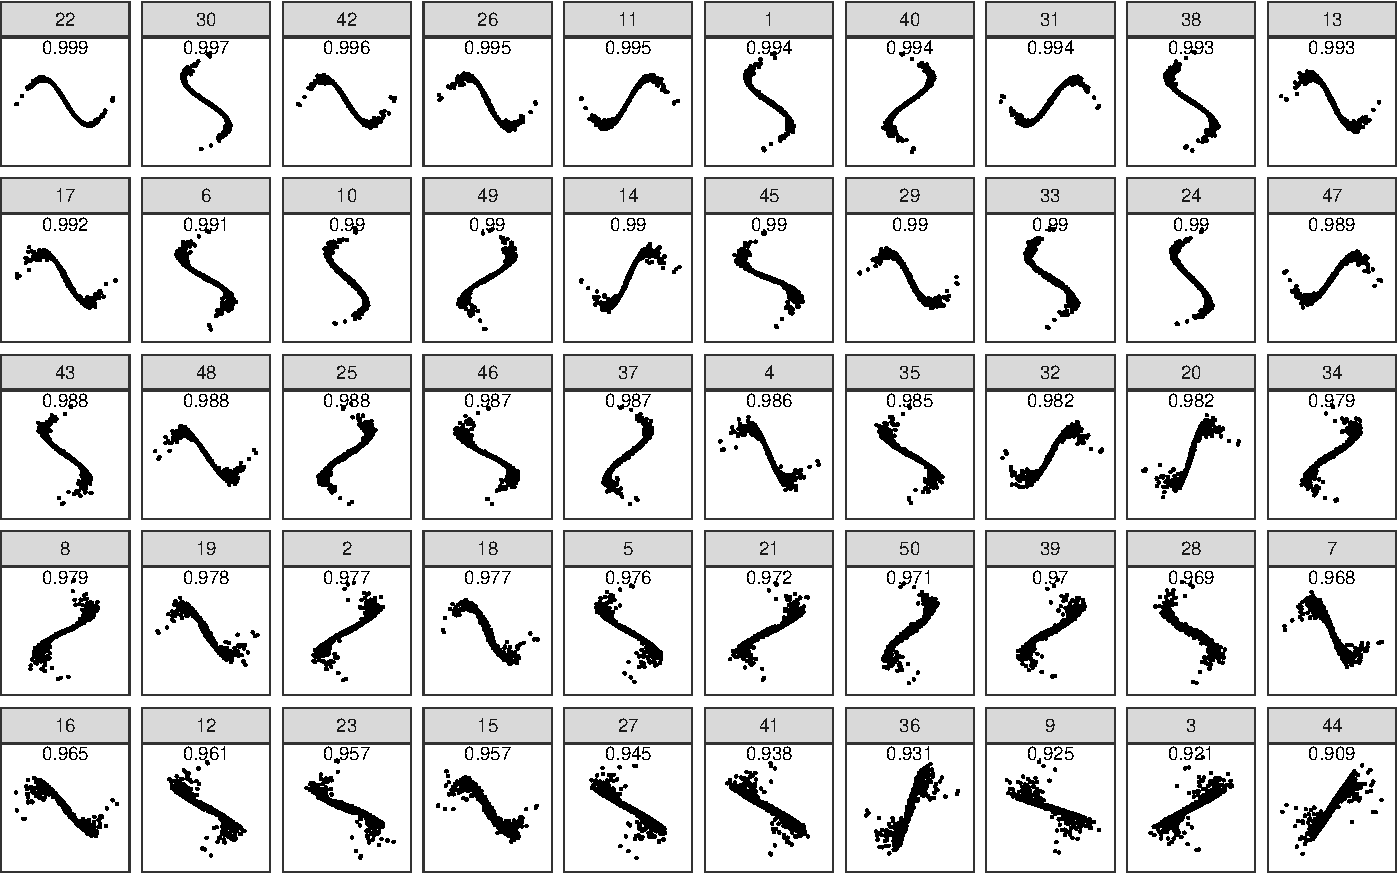
\includegraphics{optim_files/figure-pdf/fig-projection-1.pdf}

}

\caption{\label{fig-projection}Best projections found by the JS
opitmiser in each simulation, sorted by the index value. The projection
pursuit problem is to detect the 6D sine-wave structure using the spline
index. Most simulations have detected a clear sine-wave pattern, while
the last six show a straight line with clustering at the ends.. In this
simulation, the success rate is 0.88 (44/50).}

\end{figure}

\begin{figure}

{\centering 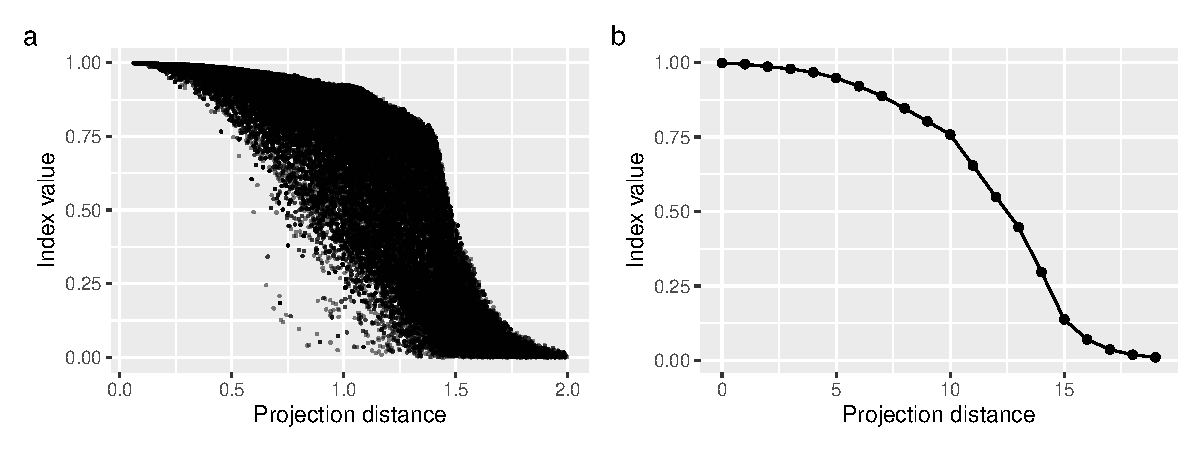
\includegraphics{optim_files/figure-pdf/fig-index-value-proj-dist-1.pdf}

}

\caption{\label{fig-index-value-proj-dist}Projection distance plotted
against the index value for detecting the 6D sine-wave structure using
the spline index function. a) The index values start around 0 with low
variance at large projection distances. As the projection distance
decreases, the index values increase with a larger variance. Towards the
minimum projection distance, the index values increase and cluster
around 1, indicating the optimiser is approaching to the optimum. b)
Projection distances are binned with a bin width of 0.1, and index
values are averaged over each bin. The relationship between the two
variables forms a sigmoid curve.}

\end{figure}

\hypertarget{sec-app}{%
\section{Application {[}Di and Sherry{]}}\label{sec-app}}

The JS optimiser provides a new swarm-based search strategy to optimise
projection pursuit problems. Two examples are provided in this section
to demonstrate its performance. The first example compares its
performance with the search-better optimiser and explores how it behaves
with different combinations of hyper-parameters. The second example
studies the effect of optimisation properties defined in
Section~\ref{sec-theory}, along with jellyfish hyper-parameters, on the
outcome of the optimisation.

\hypertarget{sec-app-1}{%
\subsection{Performance of the JS optimiser in pipe-finding
problems}\label{sec-app-1}}

The performance of the JS optimiser is investigated in two folds: 1)
compare it with a commonly used optimiser: the search-better optimiser
\citep{RJ-2021-105, laa_using_2020}, and 2) examine its success rate
under different hyper-parameters (number of jellyfishes and maximum
number of tries). The projection pursuit problem used is finding the
pipe shape using the holes index, investigated by
\citet{laa_using_2020}.

\begin{figure}

{\centering \includegraphics{optim_files/figure-pdf/fig-proj-1.pdf}

}

\caption{\label{fig-proj}Projections found by the jellyfish and search
better optimisers at each 10th quantile across 50 simulations. The
projection pursuit problem is to find the pipe shape using the holes
index in the 6, 8, 10, and 12-dimensional spaces. The JS optimiser uses
100 jellyfishes and a maximum number of tries of 100. The search better
optimiser uses a maximum of 1000 tries in each step of random sampling
step before the algorithm terminates. In the 6-D data space, the JS
optimiser always finds a clear pipe shape while the search better
optimiser also finds the pipe shape but with a wide rim. At higher data
dimensions, the JS optimiser finds a higher index value and a clearer
pipe shape across all the quantiles than the search better optimiser.}

\end{figure}

\begin{figure}

{\centering 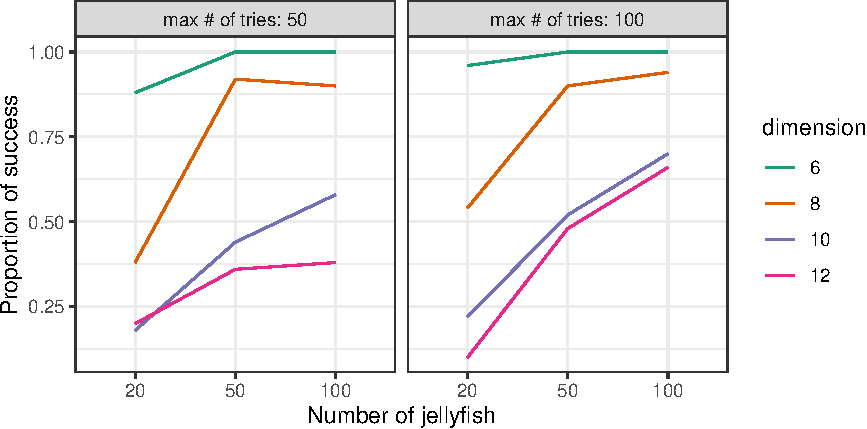
\includegraphics{optim_files/figure-pdf/fig-proportion-1.pdf}

}

\caption{\label{fig-proportion}Proportion of simulations reaches
near-optimal index values in the pipe-finding problem using the holes
index. The proportion is calculated based on the number of simulations,
out of 50, that achieve an index value within 0.05 of the
best-performing simulation. As the dimensionality increases, the
proportion of simulations reaching the optimal index value increases.}

\end{figure}

Fifty simulations are conducted with both JS and the search-better
optimiser, in four dimensions (\(d = 6, 8, 10, 12\)). The JS optimiser
uses 100 jellyfishes and 100 maximum number of tries, while the
search-better optimiser allows a maximum of 1000 samples at each
iteration before the algorithm terminates. Figure~\ref{fig-proj}
presents the final projections found by the two optimisers, broken down
by 10th quantile, faceted by the data dimension. In the 6-dimensional
data scenario, the JS optimiser consistently identifies a clear pipe
shape. The search-better optimiser also finds the pipe shape but with a
wide rim, suggesting a further polish search may be required. With
increasing dimensions, the JS optimiser may not always identify the pipe
shape due to random sampling, but it still presents a pipe shape in over
50\% of cases. When compared to the search-better optimiser, the JS
optimiser reaches higher index values and clearer pipe shapes across all
quantiles.

In the second experiment, fifty simulations are conducted at each
hyper-parameter combination to analyse its effects on the success rate
of the JS optimiser. The hyper-parameters tested include: 1) 20, 50, and
100 jellyfishes, and 2) 50 and 100 maximum number of tries. In each
simulation, the success rate is calculated as defined in
Section~\ref{sec-vis}. Figure~\ref{fig-proportion} presents the
proportion of success for each hyper-parameter combinations. As the
number of jellyfishes and maximum tries increase, the success rate also
increases. For simpler problems (6 dimensions), small parameter values
(20 jellyfishes and a maximum number of tries of 50) can already result
in high success rate, while for higher-dimensional problems (8, 10, and
12 dimensions), a combination of 100 jellyfishes and 100 maximum number
of tries is necessary for at least half of the jellyfishes to find the
optimal projection.

\hypertarget{sec-app-2}{%
\subsection{Factors affecting the JS optimiser success rate:
optimisation properties and jellyfish
hyper-parameters}\label{sec-app-2}}

The optimisation properties, including smoothness, squintability, and
speed, offer numerical metrics to characterise the complexity of a
projection pursuit optimisation problem. This example investigates how
these metrics, along with the jellyfish search hyper-parameters (the
number of jellyfishes and the maximum number of tries), affect the
success of the JS optimiser. Simulations are conducted to obtain the
success rate across various projection pursuit problems, characterised
by shape-to-find, data dimension, and index function used, as well as
different hyper-parameter combinations. Smoothness and squintability are
calculated for each projection pursuit problem as outlined in
Section~\ref{sec-theory}. A generalised linear model is used to
construct the relationship between the success rate, jellyfish
hyper-parameters and optimisation properties.

In addition to the pipe-finding problem, a new shape, sine wave, is
investigated in 6D and 8D spaces with six indices considered:
\texttt{dcor2d\_2}, \texttt{loess2d}, \texttt{MIC}, \texttt{TIC},
\texttt{spline}, and \texttt{stringy}. Combining with two jellyfish
hyper-parameters, a total of 52 cases is produced, comprising of 24
pipe-finding cases and 28 sine-wave finding cases. For each case, the JS
optimiser is run fifty times and the success rate is calculated as in
Section~\ref{sec-app-1}.

Smoothness and squintability are computed for each case, following the
procedures outlined in Section~\ref{sec-smoothness} and
Section~\ref{sec-squintability}. To calculate smoothness, three hundred
random bases are simulated. Index values and projection distance (to the
optimal basis) are calculated for each random basis before fitting them
into a Gaussian process model. For squintability, fifty random bases are
sampled and interpolated to the optimal basis with a step size of 0.005.
For these interpolated bases, index values and projection distances to
the optimal basis are calculated and averaged with a bin width of 0.005.
The squintability measure is then calculated from fitting a 4-parameter
scaled logistic function of index value against projection distance,
estimated by non-linear least squares.

Table~\ref{tbl-smoothness-squintability} presents the parameters
estimated from the Gaussian process (variance, range, smooth, and
nugget) and the scaled logistic function (\(\theta_1\) to \(\theta_4\))
for each case. The column ``smooth'' is used as the smoothness measure
and the column ``squint'' is calculated as {[}TODO: equation
reference{]} as squintability. The low squint value of MIC and TIC index
is due to its convex shape of the index value against the projection
distance, as shown in Figure~\ref{fig-idx-proj-dist}. Comparing to other
concave shapes, the maximum first derivative happens at a smaller
projection distance (\(\theta_2\)), requiring the optimiser to get
closer to the optimal to see a significant change in the index value,
hence a small squintability measure.

\begin{figure}

{\centering 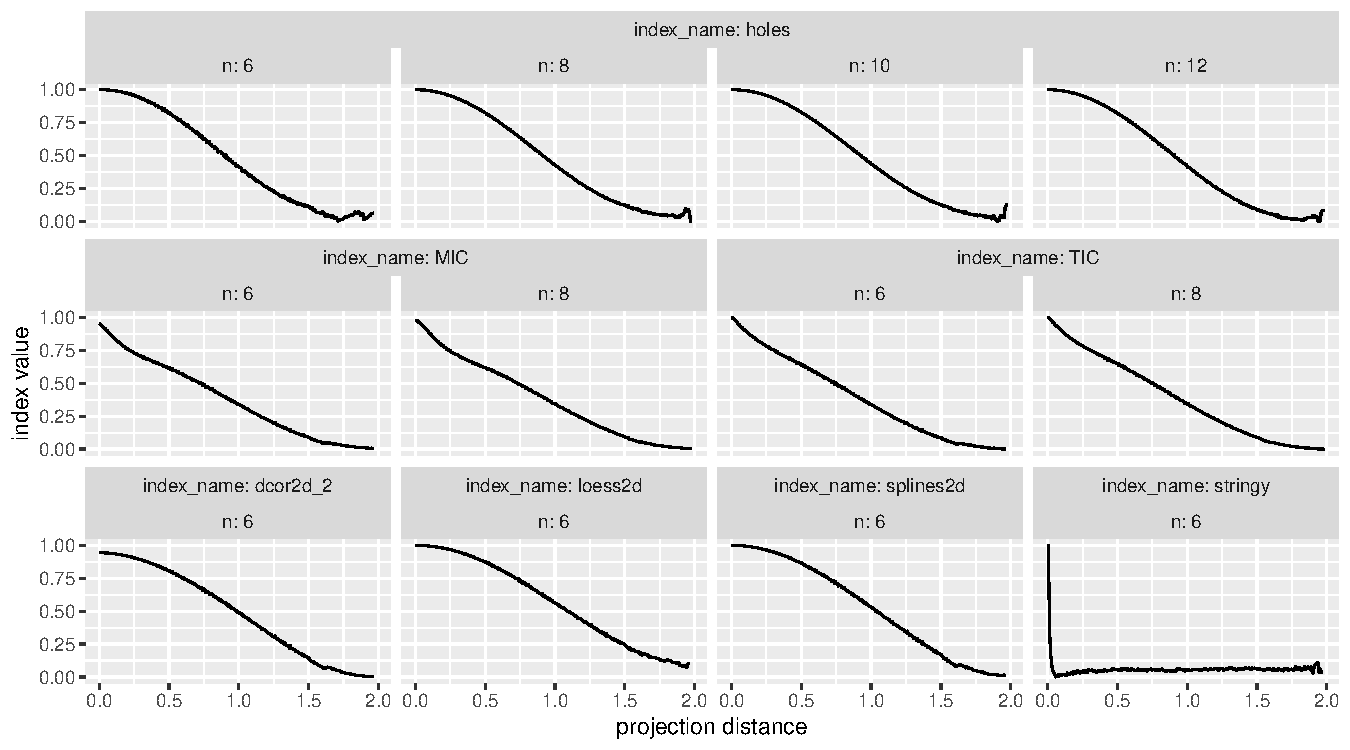
\includegraphics{optim_files/figure-pdf/fig-idx-proj-dist-1.pdf}

}

\caption{\label{fig-idx-proj-dist}Index values versus projection
distance for the 12 pipe/sine-wave finding problem, after the binning
procedure for calculating the squintability measure. The index values,
averaged at bin width of 0.005, are scaled from 0 to 1 for comparison
(holes, TIC, and stringy). The \texttt{MIC} and \texttt{TIC} index
curves are convex while others are concave. The stringy curve shows an
instantaneous jump to the optimum when aproaching the best basis.}

\end{figure}

Table~\ref{tbl-mod-data} combines all the variables calculated above
(the JS optimiser success rate, jellyfish hyper-parameters, and
optimisation properties) into one table. Three preprocessing steps are
applied to the data: 1) scaling the jellyfish hyper-parameters by a
factor of 10 for interpretation, 2) creating a new binary variable
\texttt{long\_time} to indicate cases with an average run time over 30
seconds, and 3) encoding the success rate for the stringy case as 0,
since none of the 50 simulations identified the sine-wave shape. A
generalised linear model with a binomial family and a logit link
function is used to fit the data and Table~\ref{tbl-mod-output} presents
the model outputs. The model suggests that the success rate of the JS
optimiser is positively associated with the two jellyfish
hyper-parameters, as well as with smoothness and squintability. However,
being flagged with long runtime and an increase of data dimension will
reduce the success rate. The variable \texttt{squintability} and
\texttt{dimension} are significant, suggesting their importance relative
to jellyfish hyper-parameters in the optimisation success.

\hypertarget{tbl-smoothness-squintability}{}
\begin{table}
\caption{\label{tbl-smoothness-squintability}Parameters estimated from the Gaussian process (including variance,
range, smoothness, and nugget) and scaled logistic function
(\(\theta_1\) to \(\theta_4\)) for the pipe-finding and sine-wave
finding problems. The column ``smooth'' and ``squint'' represent the
smoothness and squintability measures. }\tabularnewline

\centering\begingroup\fontsize{7}{9}\selectfont

\begin{tabular}{|>{}lll>{}r|rrr>{}r|rrr>{}r|>{}r|}
\toprule
  & shape & index & d & variance & range & smooth & nugget & $\theta_1$ & $\theta_2$ & $\theta_3$ & $\theta_4$ & squint\\
\midrule
1 & pipe & holes & 6 & 0.002 & 0.371 & 2.355 & 0.221 & 1.015 & 0.860 & 3.368 & 0.018 & 0.763\\
2 & pipe & holes & 8 & 0.000 & 0.178 & 2.189 & 0.820 & 1.014 & 0.869 & 3.264 & 0.029 & 0.740\\
3 & pipe & holes & 10 & 0.000 & 0.107 & 2.192 & 3.027 & 1.016 & 0.885 & 3.151 & 0.022 & 0.737\\
4 & pipe & holes & 12 & 0.000 & 0.148 & 2.295 & 1.581 & 1.011 & 0.878 & 3.345 & 0.004 & 0.779\\
5 & sine & MIC & 6 & 0.016 & 0.092 & 2.457 & 0.083 & 0.894 & 0.571 & 1.623 & -0.024 & 0.314\\
\addlinespace
6 & sine & MIC & 8 & 0.016 & 0.081 & 2.636 & 0.084 & 0.932 & 0.328 & 1.314 & -0.030 & 0.193\\
7 & sine & TIC & 6 & 0.124 & 0.110 & 2.444 & 0.086 & 0.951 & 0.536 & 1.719 & -0.027 & 0.330\\
8 & sine & TIC & 8 & 0.125 & 0.099 & 2.475 & 0.085 & 0.949 & 0.564 & 1.723 & -0.028 & 0.342\\
9 & sine & dcor2d & 6 & 0.034 & 0.167 & 2.663 & 0.114 & 0.954 & 1.039 & 2.742 & -0.019 & 0.737\\
10 & sine & loess2d & 6 & 0.079 & 0.336 & 1.988 & 0.309 & 1.016 & 1.039 & 2.648 & 0.080 & 0.689\\
\addlinespace
11 & sine & splines2d & 6 & 0.042 & 0.242 & 2.537 & 0.102 & 1.014 & 1.051 & 2.730 & -0.009 & 0.780\\
12 & sine & stringy & 6 & 0.000 & 0.007 & 1.536 & 38.166 & 1.045 & 0.011 & 254.734 & 0.053 & 0.739\\
\bottomrule
\end{tabular}
\endgroup{}
\end{table}

\begingroup\fontsize{7}{9}\selectfont

\hypertarget{tbl-mod-data}{}
\begin{longtable}[t]{lrrrrrrl}
\caption{\label{tbl-mod-data}The first 7 rows of the datasets processed for modelling. }\tabularnewline

\toprule
Index & D & Smoothness & Squintability & Num. of jellyfish & Max. Num. of tries & Prop. of success & Time\\
\midrule
MIC & 6 & 2.457 & 0.314 & 20 & 50 & 0.12 & 2.479 secs\\
MIC & 6 & 2.457 & 0.314 & 20 & 100 & 0.24 & 8.950 secs\\
MIC & 6 & 2.457 & 0.314 & 50 & 50 & 0.52 & 5.651 secs\\
MIC & 6 & 2.457 & 0.314 & 50 & 100 & 0.64 & 13.223 secs\\
MIC & 6 & 2.457 & 0.314 & 100 & 50 & 0.76 & 19.453 secs\\
\addlinespace
MIC & 8 & 2.636 & 0.193 & 20 & 50 & 0.08 & 2.566 secs\\
MIC & 8 & 2.636 & 0.193 & 20 & 100 & 0.08 & 4.960 secs\\
\bottomrule
\end{longtable}
\endgroup{}

\begingroup\fontsize{7}{9}\selectfont

\hypertarget{tbl-mod-output}{}
\begin{longtable}[t]{|>{}lrrr>{}r|}
\caption{\label{tbl-mod-output}Model estimates of proportion of jellyfish success on optimisation
properties and jellyfish hyper-parameters from the generalised linear
model with a binomial family and a logit link function. The variable
smoothness, squintability, number of jellyfish and maximum number of
tries are positively associated with the JS optimiser success rate while
data dimension and being flagged as long runtime are negatively
associated with the success rate. The variable squintability and
dimension are significant, suggesting their importance relative to
jellyfish hyper-parameters in the optimisation success. }\tabularnewline

\toprule
term & estimate & std.error & statistic & p.value\\
\midrule
Intercept & -4.523 & 5.332 & -0.848 & 0.396\\
Smoothness & 1.195 & 1.915 & 0.624 & 0.533\\
Squintability & 8.241 & 2.737 & 3.011 & 0.003\\
dimension (d) & -0.628 & 0.255 & -2.462 & 0.014\\
long time & -0.874 & 1.286 & -0.680 & 0.497\\
\addlinespace
number of jellyfish & 0.216 & 0.127 & 1.701 & 0.089\\
maximum number of tries & 0.113 & 0.150 & 0.752 & 0.452\\
\bottomrule
\end{longtable}
\endgroup{}

\hypertarget{sec-conclusion}{%
\section{Conclusion {[}Di and Sherry{]}}\label{sec-conclusion}}


\renewcommand\refname{References}
  \bibliography{bibliography.bib}


\end{document}
